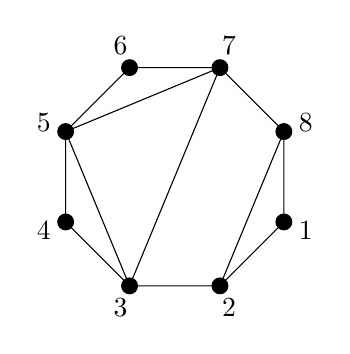
\begin{tikzpicture}
\def \n {1}
\def \R {1.5cm}
\def \RR {1.8cm}
\def \one {-22.5}
\def \two {-67.5}
\def \three {-112.5}
\def \four {-157.5}
\def \five {-202.5}
\def \six {-247.5}
\def \seven {-292.5}
\def \eight {-337.5}
\draw (-22.5:\R) \foreach \x in {-67.5,-112.5,-157.5,-202.5,-247.5,-292.5,-337.5} {
            -- (\x:\R)
        } -- cycle;
\foreach \x in {-22.5,-67.5,-112.5,-157.5,-202.5,-247.5,-292.5,-337.5} {
        \draw [fill] (\x:\R)  circle [radius=0.1];
        }
\foreach \x/\i in {-22.5/1,-67.5/2,-112.5/3,-157.5/4,-202.5/5,-247.5/6,-292.5/7,-337.5/8} {
        \node at (\x:\RR) {\i};
        }
\draw (\seven:\R) -- (\three:\R) -- (\five:\R) -- cycle;
\draw (\eight:\R) -- (\two:\R);
\end{tikzpicture}
